\documentclass[transfermodule]{naklatex}

%Literatur Einstellungen
\usepackage[backend=biber, style=authoryear, hyperref=true, natbib=true, maxbibnames=9, maxcitenames=2]{biblatex}
\usepackage{color}
\DefineBibliographyStrings{ngerman}{
        andothers = {{et\,al\adddot}},
}
\ExecuteBibliographyOptions{sorting=nty}
\addbibresource{quellen.bib}

%import glossaries files
\loadglsentries{content/glossary.tex}
\loadglsentries{content/acronym.tex}

\begin{document}
	\hypersetup{pageanchor=false}

	\title{Arbeit}
	\studentnumber{12345}
	\class{A16a}
	\thema{Das ist das Thema der TL}
	\transfermodulenumber{3}

	\maketitle

	\thispagestyle{empty}

\setlength{\parindent}{0pt}

\begin{figure}[t]
	\vspace*{-2.9\baselineskip}
	\begin{subfigure}[b]{0.6\textwidth}
		
\includegraphics[height=1cm, left]{image/transferleistung}
	\end{subfigure}
	\begin{subfigure}[b]{0.4\textwidth}
		
\includegraphics[height=1.4cm, right]{image/nak_new_logo_big}
	\end{subfigure}
\end{figure}
\begin{figure}[t]
	\begin{tikzpicture}
		\fill[blue!35!black,path fading=west] (0,-0.5pt) rectangle (\linewidth,0.5pt);
	\end{tikzpicture}
\end{figure}


\large
\textcolor{blue!30!black}{\textbf{Transferleistung Theorie/Praxis }}
\transfermodulenumber
\newline\newline

\normalsize
\begin{tabular}{ |p{5cm}|p{11cm}| }
    \hline
    \cellcolor{blue!35!black}\textcolor{white}{\textbf{Matrikelnummer:}\newline} &\studentnumber \\
    \hline
    \cellcolor{blue!35!black}\textcolor{white}{\textbf{Freigegebenes Thema:}\newline\newline\newline\newline} &\thema \\
    \hline
    \cellcolor{blue!35!black}\textcolor{white}{\textbf{Studiengang, Zenturie:}\newline} &\class \\

    \hline
\end{tabular}

	%\pagebreak
\thispagestyle{empty}

\setlength{\parindent}{0pt}

\begin{figure}[t]
	\vspace*{-2.9\baselineskip}
	\begin{subfigure}[b]{0.6\textwidth}
		
\includegraphics[height=1cm, left]{image/transferleistung}
	\end{subfigure}
	\begin{subfigure}[b]{0.4\textwidth}
		
\includegraphics[height=1.4cm, right]{image/nak_new_logo_big}
	\end{subfigure}
\end{figure}
\begin{figure}[t]
	\begin{tikzpicture}
		\fill[blue!35!black,path fading=west] (0,-0.5pt) rectangle (\linewidth,0.5pt);
	\end{tikzpicture}
\end{figure}


\vspace*{\fill}

\large
\textcolor{blue!30!black}{\textbf{Eidesstattliche Erklärung des Studenten / der Studentin }}
\newline

\normalsize
Hiermit erkläre ich an Eides statt, dass ich die vorliegende Arbeit ohne Hilfe Dritter und ohne
Benutzung anderer als der angegebenen Hilfsmittel angefertigt habe. Die aus fremden
Quellen direkt oder indirekt übernommenen Gedanken sind als solche kenntlich gemacht.
Die Arbeit wurde bisher in gleicher oder ähnlicher Form weder von mir noch von jemand
anderem als Prüfungsleistung vorgelegt.
\newline

\begin{tabular}{ p{1.2cm}p{4.5cm}p{2cm}p{2cm}p{4.5cm} }
    Datum: & \today & & Unterschrift: & 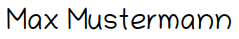
\includegraphics[height=20px]{image/signature.png}\\\cline{2-2}\cline{5-5}
\end{tabular}

\vspace*{\fill}


	%\pagebreak
\thispagestyle{empty}

\setlength{\parindent}{0pt}

\begin{figure}[t]
	\vspace*{-2.9\baselineskip}
	\begin{subfigure}[b]{0.6\textwidth}
		
\includegraphics[height=1cm, left]{image/transferleistung}
	\end{subfigure}
	\begin{subfigure}[b]{0.4\textwidth}
		
\includegraphics[height=1.4cm, right]{image/nak_new_logo_big}
	\end{subfigure}
\end{figure}
 
\begin{figure}[t]
	\begin{tikzpicture}
		\fill[blue!35!black,path fading=west] (0,-0.5pt) rectangle (\linewidth,0.5pt);
	\end{tikzpicture}
	
\end{figure}

\vspace*{\fill}

\large
\textcolor{blue!30!black}{\textbf{Sperrvermerk}}
\newline

\normalsize
Die vorliegende Hausarbeit mit dem Titel \textbf{Transferleistung Theorie/Praxis Nr.2}
beinhaltet interne und vertrauliche Informationen des Unternehmens \textbf{Otto (GmbH \& Co KG)}.
	
Die Weitergabe des Inhalts der Arbeit und eventuell beiliegender Zeichnungen und Daten, im Gesamten oder in Teilen, ist grundsätzlich untersagt. Es dürfen keinerlei Kopien oder Abschriften – auch in digitaler Form – gefertigt werden. Ausnahmen bedürfen der schriftlichen Genehmigung des Unternehmens.

	Hamburg, den \today

\vspace*{\fill}

	\pagebreak
\thispagestyle{empty}

\setlength{\parindent}{0pt}

\begin{figure}[t]
	\vspace*{-2.9\baselineskip}
	\begin{subfigure}[b]{0.6\textwidth}
		
\includegraphics[height=1cm, left]{image/transferleistung}
	\end{subfigure}
	\begin{subfigure}[b]{0.4\textwidth}
		
\includegraphics[height=1.4cm, right]{image/nak_new_logo_big}
	\end{subfigure}
\end{figure}
\begin{figure}[t]
	\begin{tikzpicture}
		\fill[blue!35!black,path fading=west] (0,-0.5pt) rectangle (\linewidth,0.5pt);
	\end{tikzpicture}
\end{figure}


\vspace*{\fill}

\large
\textcolor{blue!30!black}{\textbf{Hinweis zur gendergerechten Sprache}}
\newline

\normalsize
Aus Gründen der besseren Lesbarkeit wird in der vorliegenden Transferleistung bei Personenbezeichnungen und personenbezogenen Hauptwörtern das generische Maskulinum verwendet. Entsprechende Begriffe sind im Sinne der Gleichbehandlung grundsätzlich als geschlechtsneutral zu verstehen, die verkürzte Sprachform beinhaltet keine Wertung.

\vspace*{\fill}


	\hypersetup{pageanchor=true}
	\pagestyle{scrheadings}
	\frontmatter 
	\tableofcontents
	\printglossaries

	\lstlistoflistings
	{\let\clearpage\relax \listoffigures}
	{\let\clearpage\relax \listoftables}

	\mainmatter
	\chapter{Einleitung}
\section{Unterteil}
Lorem ipsum dolor sit amet, consetetur sadipscing, sed diam nonumy Transferleistung Transferleistung tempor invidunt ut labore et dolore magna aliquyam erat, sed diam voluptua. At vero eos et accusam et justo duo dolores et ea rebum. Stet clita kasd gubergren, no sea takimata sanctus est Lorem ipsum dolor sit amet. Lorem ipsum dolor sit amet, consetetur sadipscing elitr, sed diam nonumy eirmod tempor invidunt ut labore et dolore magna aliquyam erat, sed diam voluptua. At vero eos et accusam et justo duo dolores et ea rebum. Stet clita kasd gubergren, no sea takimata sanctus est Lorem ipsum dolor sit amet. Lorem ipsum dolor sit amet, consetetur sadipscing elitr, sed diam nonumy eirmod tempor invidunt ut labore et dolore magna aliquyam erat, sed diam voluptua. At vero eos et accusam et justo duo dolores et ea rebum. Stet clita kasd gubergren, no sea takimata sanctus est Lorem ipsum dolor sit amet.

\section{Unterteil 2}
Duis autem vel eum iriure dolor in hendrerit in vulputate velit esse molestie consequat, vel illum dolore eu feugiat nulla facilisis at vero eros et accumsan et iusto odio dignissim qui blandit praesent luptatum zzril delenit augue duis dolore te feugait nulla facilisi. Lorem ipsum dolor sit amet,
	\chapter{Figuren}
\section{Bild}
Bildern können Unterschriften hinzugefügt werden. Außerdem kann auf die bilder verwiesen werden (siehe \autoref{fig:image1})
\begin{figure}[htbp]
	\centering
	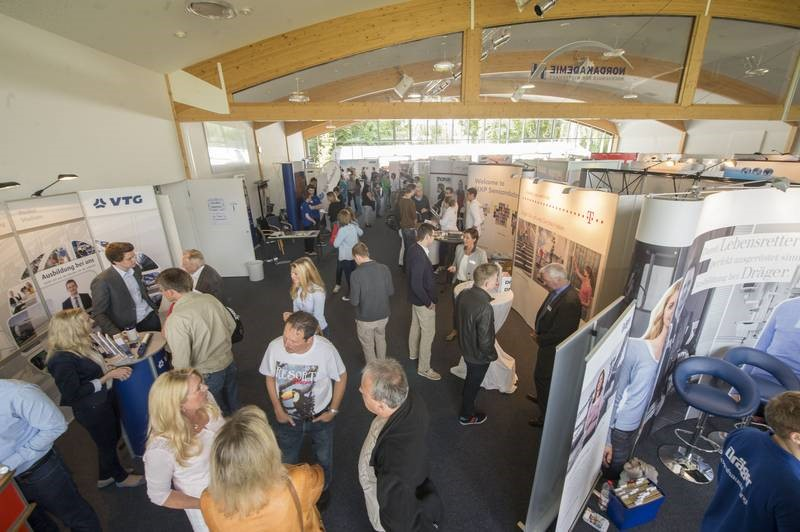
\includegraphics[width=0.9\linewidth]{image/image1}
	\caption[Nordakademie 14. Studieninformationstag]{Nordakademie 14. Studieninformationstag}
	\label{fig:image1}
\end{figure}
\section{Tabelle}
Auch Tabellen sind toll.
\begin{lstlisting}[
    caption={Testy},
    mathescape=true,showstringspaces=false,
    flexiblecolumns=true,
    tabsize=2,
    numbersep=1pt,
    numbers=left,
    xleftmargin=0.2cm,
    framerule=0pt
    ]
  import java.util.Date;
    
  val a: String = "testy"
    
  /*
  * Bildet vereinfacht eine Person mittels einer Datenklasse in Kotlin ab.
  */

  @Testy 
  data class Person(var vorname: String, var nachname: String, 
                      var alter: Int, var geburtsdatum: Date)    
\end{lstlisting}

\begin{table}[htbp]
	\centering
    \begin{tabular}{|l|l|l|}
    \hline
    Überschrift1 & 2 & 3 \\ \hline
    ef &  & dfdf \\ \hline
    dfg & f & fgb \\ \hline
    gfp & fg &  \\ \hline
    f &  &  \\ \hline
    juhz &  & rt \\ \hline
    rtg &  & ikiu \\ \hline
    \end{tabular}
    \caption{Beispieltabelle} 
    \label{table:Tabelle}
\end{table}

\chapter{Glossar}
Es wird zwischen Worterklärungen (Glossar) und Abkürzungen (Akronymen) unterschieden.
\section{Glossar}
Dies ist ein Beispiel für ein Eintrag im \Gls{glossar}. Das Wort kann auch im Plural ausgegeben werden (\Glspl{glossar}).
\section{Akronyme}
\gls{latex} wird automatisch bei der ersten Nutzung des Akronyms die Erklärung hinzufügen. Bei späteren Erwähnungen wird \gls{latex} nur die Abkürzung ausgeben.
\chapter{Literatur}
Es kann ganz einfach auf eine Quelle verwiesen werden \autocite{blubb}

	\printbibliography[title={Literaturverzeichnis}]

	\appendix
	\chapter{Anhang}
\section{Übersicht über folgende Blubb}
Lorem ipsum dolor sit amet, consetetur sadipscing elitr, sed diam nonumy eirmod tempor invidunt ut labore et dolore magna aliquyam erat, sed diam voluptua. At vero eos et accusam et justo duo dolores et ea rebum. Stet clita kasd gubergren, no sea takimata sanctus est Lorem ipsum dolor sit amet. Lorem ipsum dolor sit amet, consetetur sadipscing elitr, sed diam nonumy eirmod tempor invidunt ut labore et dolore magna aliquyam erat, sed diam voluptua. At vero eos et accusam et justo duo dolores et ea rebum. Stet clita kasd gubergren, no sea takimata sanctus est Lorem ipsum dolor sit amet.

Lorem ipsum dolor sit amet, consetetur sadipscing elitr, sed diam nonumy eirmod tempor invidunt ut labore et dolore magna aliquyam erat, sed diam voluptua. At vero eos et accusam et justo duo dolores et ea rebum. Stet clita kasd gubergren, no sea takimata sanctus est Lorem ipsum dolor sit amet. Lorem ipsum dolor sit amet, consetetur sadipscing elitr, sed diam nonumy eirmod tempor invidunt ut labore et dolore magna aliquyam erat, sed diam voluptua. At vero eos et accusam et justo duo dolores et ea rebum. Stet clita kasd gubergren, no sea takimata sanctus est Lorem ipsum dolor sit amet.Lorem ipsum dolor sit amet, consetetur sadipscing elitr, sed diam nonumy eirmod tempor invidunt ut labore et dolore magna aliquyam erat, sed diam voluptua. At vero eos et accusam et justo duo dolores et ea rebum. Stet clita kasd gubergren, no sea takimata sanctus est Lorem ipsum dolor sit amet. Lorem ipsum dolor sit amet, consetetur sadipscing elitr, sed diam nonumy eirmod tempor invidunt ut labore et dolore magna aliquyam erat, sed diam voluptua. At vero eos et accusam et justo duo dolores et ea rebum. Stet clita kasd gubergren, no sea takimata sanctus est Lorem ipsum dolor sit amet.

Lorem ipsum dolor sit amet, consetetur sadipscing elitr, sed diam nonumy eirmod tempor invidunt ut labore et dolore magna aliquyam erat, sed diam voluptua. At vero eos et accusam et justo duo dolores et ea rebum. Stet clita kasd gubergren, no sea takimata sanctus est Lorem ipsum dolor sit amet. Lorem ipsum dolor sit amet, consetetur sadipscing elitr, sed diam nonumy eirmod tempor invidunt ut labore et dolore magna aliquyam erat, sed diam voluptua. At vero eos et accusam et justo duo dolores et ea rebum. Stet clita kasd gubergren, no sea takimata sanctus est Lorem ipsum dolor sit amet.Lorem ipsum dolor sit amet, consetetur sadipscing elitr, sed diam nonumy eirmod tempor invidunt ut labore et dolore magna aliquyam erat, sed diam voluptua. At vero eos et accusam et justo duo dolores et ea rebum. Stet clita kasd gubergren, no sea takimata sanctus est Lorem ipsum dolor sit amet. Lorem ipsum dolor sit amet, consetetur sadipscing elitr, sed diam nonumy eirmod tempor invidunt ut labore et dolore magna aliquyam erat, sed diam voluptua. At vero eos et accusam et justo duo dolores et ea rebum. Stet clita kasd gubergren, no sea takimata sanctus est Lorem ipsum dolor sit amet.

Lorem ipsum dolor sit amet, consetetur sadipscing elitr, sed diam nonumy eirmod tempor invidunt ut labore et dolore magna aliquyam erat, sed diam voluptua. At vero eos et accusam et justo duo dolores et ea rebum. Stet clita kasd gubergren, no sea takimata sanctus est Lorem ipsum dolor sit amet. Lorem ipsum dolor sit amet, consetetur sadipscing elitr, sed diam nonumy eirmod tempor invidunt ut labore et dolore magna aliquyam erat, sed diam voluptua. At vero eos et accusam et justo duo dolores et ea rebum. Stet clita kasd gubergren, no sea takimata sanctus est Lorem ipsum dolor sit amet.Lorem ipsum dolor sit amet, consetetur sadipscing elitr, sed diam nonumy eirmod tempor invidunt ut labore et dolore magna aliquyam erat, sed diam voluptua. At vero eos et accusam et justo duo dolores et ea rebum. Stet clita kasd gubergren, no sea takimata sanctus est Lorem ipsum dolor sit amet. Lorem ipsum dolor sit amet, consetetur sadipscing elitr, sed diam nonumy eirmod tempor invidunt ut labore et dolore magna aliquyam erat, sed diam voluptua. At vero eos et accusam et justo duo dolores et ea rebum. Stet clita kasd gubergren, no sea takimata sanctus est Lorem ipsum dolor sit amet.

Lorem ipsum dolor sit amet, consetetur sadipscing elitr, sed diam nonumy eirmod tempor invidunt ut labore et dolore magna aliquyam erat, sed diam voluptua. At vero eos et accusam et justo duo dolores et ea rebum. Stet clita kasd gubergren, no sea takimata sanctus est Lorem ipsum dolor sit amet. Lorem ipsum dolor sit amet, consetetur sadipscing elitr, sed diam nonumy eirmod tempor invidunt ut labore et dolore magna aliquyam erat, sed diam voluptua. At vero eos et accusam et justo duo dolores et ea rebum. Stet clita kasd gubergren, no sea takimata sanctus est Lorem ipsum dolor sit amet.Lorem ipsum dolor sit amet, consetetur sadipscing elitr, sed diam nonumy eirmod tempor invidunt ut labore et dolore magna aliquyam erat, sed diam voluptua. At vero eos et accusam et justo duo dolores et ea rebum. Stet clita kasd gubergren, no sea takimata sanctus est Lorem ipsum dolor sit amet. Lorem ipsum dolor sit amet, consetetur sadipscing elitr, sed diam nonumy eirmod tempor invidunt ut labore et dolore magna aliquyam erat, sed diam voluptua. At vero eos et accusam et justo duo dolores et ea rebum. Stet clita kasd gubergren, no sea takimata sanctus est Lorem ipsum dolor sit amet.

Lorem ipsum dolor sit amet, consetetur sadipscing elitr, sed diam nonumy eirmod tempor invidunt ut labore et dolore magna aliquyam erat, sed diam voluptua. At vero eos et accusam et justo duo dolores et ea rebum. Stet clita kasd gubergren, no sea takimata sanctus est Lorem ipsum dolor sit amet. Lorem ipsum dolor sit amet, consetetur sadipscing elitr, sed diam nonumy eirmod tempor invidunt ut labore et dolore magna aliquyam erat, sed diam voluptua. At vero eos et accusam et justo duo dolores et ea rebum. Stet clita kasd gubergren, no sea takimata sanctus est Lorem ipsum dolor sit amet.

\section{Weiteres}
Lorem ipsum dolor sit amet, consetetur sadipscing elitr, sed diam nonumy eirmod tempor invidunt ut labore et dolore magna aliquyam erat, sed diam voluptua. At vero eos et accusam et justo duo dolores et ea rebum. Stet clita kasd gubergren, no sea takimata sanctus est Lorem ipsum dolor sit amet. Lorem ipsum dolor sit amet, consetetur sadipscing elitr, sed diam nonumy eirmod tempor invidunt ut labore et dolore magna aliquyam erat, sed diam voluptua. At vero eos et accusam et justo duo dolores et ea rebum. Stet clita kasd gubergren, no sea takimata sanctus est Lorem ipsum dolor sit amet.

	\backmatter
\end{document}